\chapter{System Description}\label{systemDescription}
%One-frame Cubli is a non-linear unstable system which is capable of standing on one of its corners as long as it is properly controlled, using the inertia created in the reaction wheel present in the setup.
The system is composed of a frame and reaction wheel as the main objects to be controlled.\\
The control action is done with a brushless DC-Motor which actuates both on the frame and the wheel.\\ 
A board with a microcontroller and a motor control board are mounted on the frame through a connecting and breakout board.\\ 
The frame is fixed to a base-plate, connected with a potentiometer that can be used for direct angle measurements.\\ 
Two additional sensor breakout boards, including an integrated circuit with gyro and accelerometer, are located at the top of the frame. These are to be used for angle and velocity measurements independently of the angle of the baseplate.\\ 
A servomotor that controls the brake system is also attached, which has an arm capable of blocking the wheel by hitting one of the two break-blocks mounted on the edge of the reaction wheel.\\
The different components of the existing system can be seen in \figref{CubliParts}, where the labels correspond to table \ref{tab:TableAAUCubliComponent}.
\\
\begin{figure}[H]
	\centering
	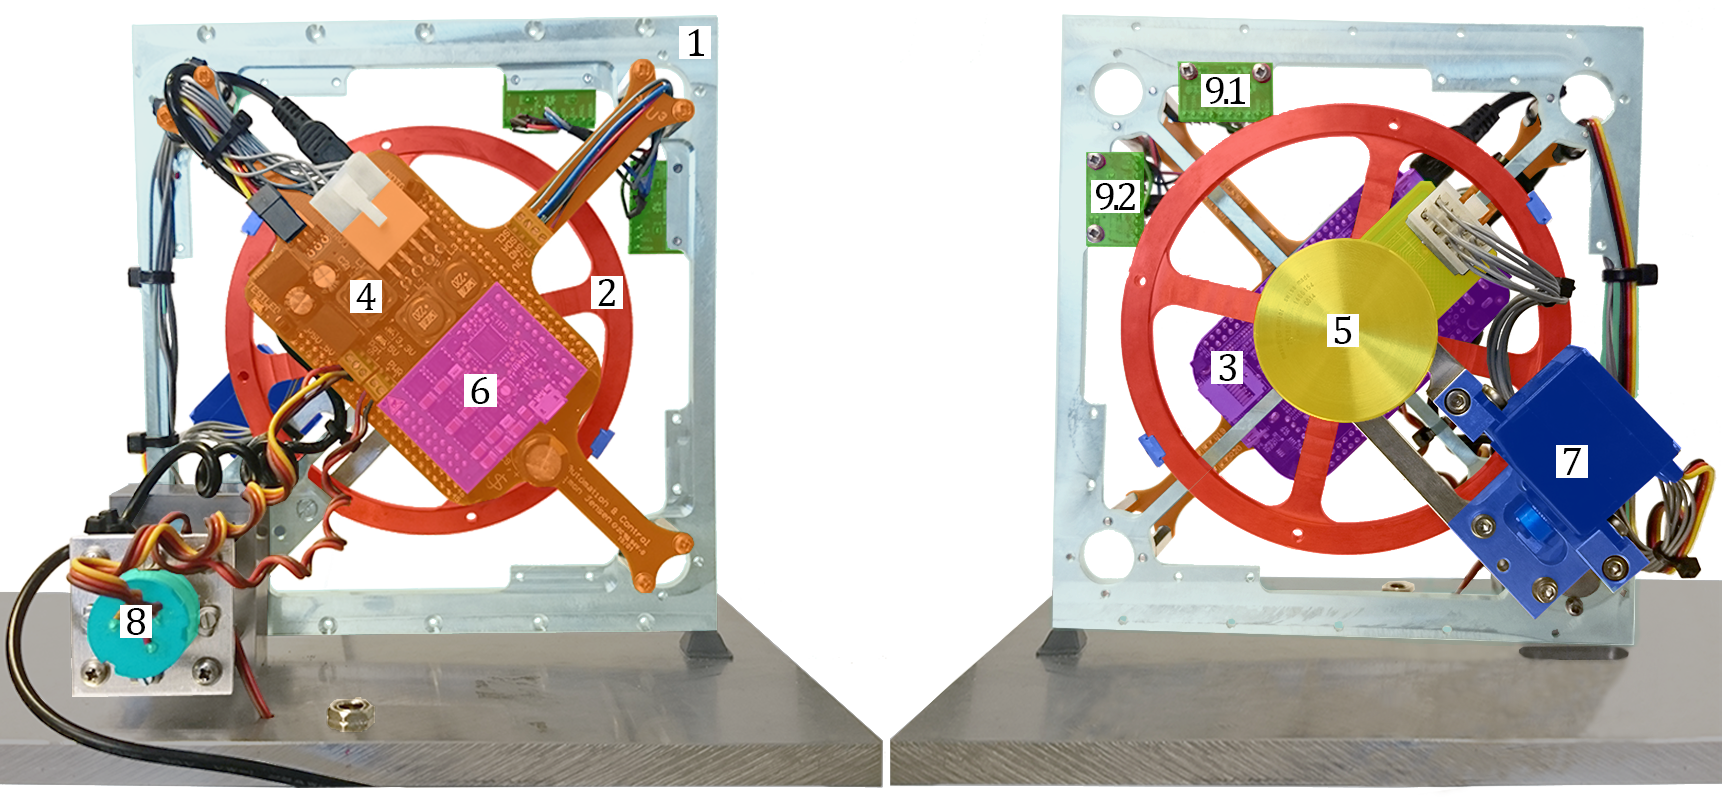
\includegraphics[scale=0.27]{figures/Cubli12}
	\caption{Existing setup viewed from the front and the back}
	\label{CubliParts}
\end{figure}
%
\begin{table}[H]
	\centering
	\begin{tabular}{|l|p{6.4cm}|}
		\hline %-----------------------------------------------------------------------------------
		\textbf{No.} &\textbf{Part} 			\\
		\hline %-----------------------------------------------------------------------------------
		1            & Frame           			\\
		\hline %-----------------------------------------------------------------------------------
		2            & Reaction Wheel      		\\
		\hline %-----------------------------------------------------------------------------------
		3            & Microcontroller (BeagleBone Black)  \\
		\hline %-----------------------------------------------------------------------------------
		4            & Connecting and Breakout Board 			\\
		\hline %-----------------------------------------------------------------------------------
		5            & Brushless DC-Motor       			\\
		\hline %-----------------------------------------------------------------------------------
		6            & Motor Control Board   	\\
		\hline %-----------------------------------------------------------------------------------
		7            & Servo Brake System     	\\
		\hline %-----------------------------------------------------------------------------------
		8            & Potentiometer 		    	\\
		\hline %-----------------------------------------------------------------------------------
		9            & Inertia Measurement Units (IMU) 		    	\\
		\hline %-----------------------------------------------------------------------------------
	\end{tabular}
	\caption{Main parts of the Cubli setup}
	\label{tab:TableAAUCubliComponent}
\end{table}
%
A detailed description of all the components, which is needed to be able to model and control the system, is presented in this chapter.

%The BeagleBone Black, the break servomotor, the Maxon motor control board and the motor itself are mounted directly on the frame. On the motor shaft a freewheel is mounted. 

%There are 2 pieces of IMU mounted on the frame to measure the acceleration and angular velocity of that frame. The latter is fixed to the platform via a potentiometer so the angular position of the frame can be measured.

%To connect the BeagleBone Black to the other units like the Maxon motor control board and the IMU and potentiometer there is a connecting and breakout board.\fxnote{Shouldn't we state who has made it ? J.}

%The Cubli at Aalborg University is a complete finished mechanical and electronic system and has been built by others.
%From the previous groups that have been working on it, some of the parameters have been found.
%To confirm and investigate the configuration of the mechanical parts changes has been made to the Cubli and the new parameters have not been measured and verified.

